\documentclass[a4paper,12pt]{report}

\usepackage{alltt, fancyvrb, url}
\usepackage{amssymb}
\usepackage{graphicx}
\usepackage{subfigure}
\usepackage{wrapfig}
\usepackage{algorithmic}
\usepackage[utf8]{inputenc}
\usepackage{fontenc}
\usepackage{amsmath,stmaryrd,mathtools,algorithm}
\usepackage{amssymb}
%\usepackage{amsfonts}
\usepackage{float}
\usepackage{hyperref}
\usepackage{listings}
\usepackage{url}

\usepackage[english]{cleveref}

\usepackage[english]{babel}

\newtheorem{definition}{Definition}[section]
\newtheorem{theorem}{Theorem}[section]
\newtheorem{property}{Property}[section]
\newcommand{\R}{\mathbb{R}}
\newcommand{\Z}{\mathbb{Z}}
\newcommand{\dd}{\cdot}

\title{Introduction to LLL\\``Cryptography''}
 
\author{Di Santi Giovanni}
\date{\today}

\begin{document}
 
\maketitle

\tableofcontents

\chapter{Linear Algebra Background}

\section{Vector Spaces}

\begin{definition}
    \textbf{Vector space}.
\end{definition}
A \texttt{vector space} $V$ is a subset of $\R^{m}$ which is closed under finite vector addition and scalar multiplication, with the property that

\begin{center}
   $a_1v_1 + a_2v_2 \in V$ for all $v_1,v_2 \in V$ and all $a_1,a_2 \in \R$
\end{center}

\begin{definition}
    \textbf{Linear Combinations}
\end{definition}

Let $v_1,v_2,\ldots,v_k \in V$. A \texttt{linear combination} of $v_1,v_2,\ldots,v_k \in V$ is any vector of the form

\begin{center}
    $\alpha_1v_1 + \alpha_2v_2 + \cdots + \alpha_kv_k$ with $\alpha_1, \ldots, \alpha_k \in \R$
\end{center}

\begin{definition}
    \textbf{Lineaer Independece}
\end{definition}

A set of vectors $v_1,v_2,\ldots,v_k \in V$ is \texttt{linearly independent} if the the only way to get

\begin{center}
    $a_1v_1 + a_2v_2 + \cdots + a_kv_k = 0$
\end{center}

is to have $a_1 = a_2 = \cdots = a_k = 0$.

\begin{definition}
    \textbf{Bases}
\end{definition}

Taken a set of linearly independent vectors $b = (v_1,\ldots,v_n) \in V$ we say that $b$ is a \texttt{basis} of $V$ if $\forall w \in V$ we can write

\begin{center}
    $w = a_1v_1 + a_2v_2 + \cdots + a_nv_n$
\end{center}

\begin{definition}
    \textbf{Vector's length}
\end{definition}

The vector's length or \texttt{Euclidean norm} of $v = (x_1, x_2, \ldots, x_m)$ is

\begin{center}
    $\lVert v \rVert = \sqrt{x_1^2 + x_2^2 + \cdots + x_m^2}$
\end{center}

\begin{definition}
    \textbf{Dot Product}
\end{definition}

Let $v, w \in V \subset \R^m$ and $v = (x_1, x_2, \ldots, x_m), w = (y_1, y_2, \ldots, y_m)$, the \texttt{dot product} of $v$ and $m$ is

\begin{center}
    $v \dd m = x_1y_1 + x_2y_2 + \cdots + x_my_m$

    or

    $v \dd m = \lVert v \rVert \lVert w \rVert \cos{\theta}$
\end{center}

where $\theta$ is the angle between $v$ and $w$ if we place the starting points of the vectors at the origin $O$.

\begin{figure}[!b]
    \centering
    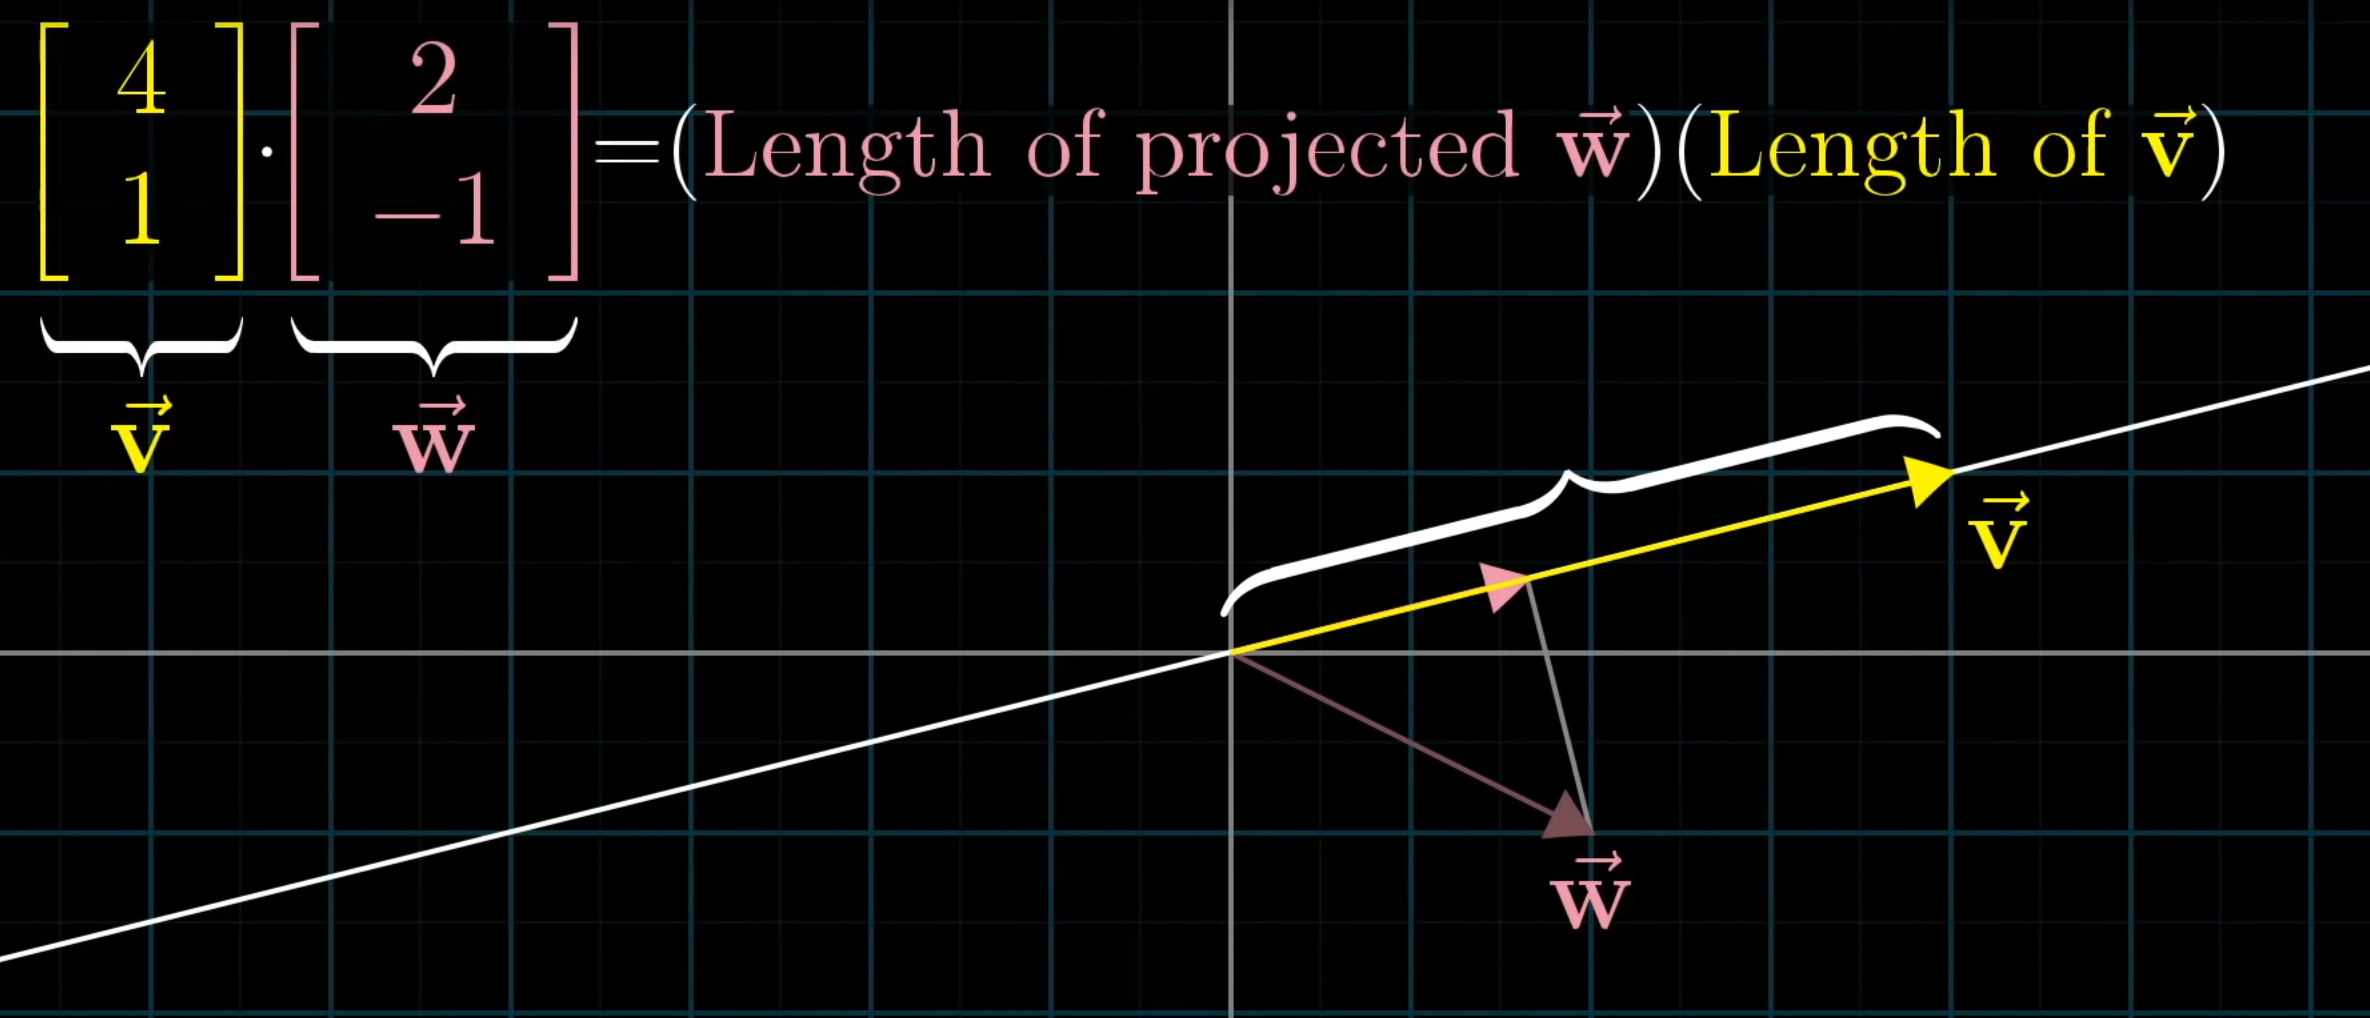
\includegraphics[scale=0.2]{./img/dot_product.png}
    \caption{Dot Product By 3Blue1Brown}
    \label{fig:dot_product}
\end{figure}

Geometrically speaking $v \cdot m$ is the length of $w$ projected to $v$ multiplied by the length of $v$ as shown in \ref{fig:dot_product}

\begin{definition}
    \textbf{Ortoghonal Basis} 
\end{definition}

An \texttt{ortoghonal basis} for a vector space $V$ is a basis $v_1, \ldots, v_m$ with the property that

\begin{center}
    $v_i \dd v_j = 0$ for all $i \neq j$
\end{center}

If $\lVert v_i \rVert = 1$ for all $i$ then the basis is \texttt{orthonormal}.

\begin{algorithm}
    \textbf{Gram-Schmidt Algorithm}
\end{algorithm}

Let $b = (v_1, \ldots, v_n)$, be a basis for a vector space $V \subset \R^m$. There is an algorithm to create an orthogonal basis
$b^* = (v_1^*,\ldots,v_n^*)$.
The two bases have the property that Span$\{v_1,\ldots,v_i\}$ = Span$\{v_1^*,\ldots,v_i^*\}$ for all $i = 1,2,\ldots,n$

\begin{figure}[htpb]
    \centering
    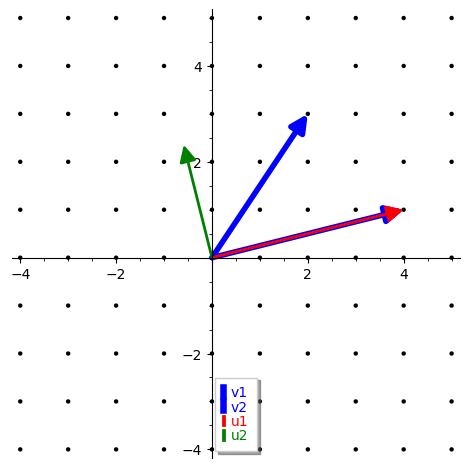
\includegraphics[width=0.5\textwidth]{./img/gram_schmidt.png}
    \caption{Gram Schmidt orthogonalization}
    \label{fig:gram_schmidt}
\end{figure}

If we take $v_1=(4, 1), v_2=(2, 3)$ as basis and apply gram schmidt we obtain $u_1=v_1=(4, 1), u_2=(-10/17, 40/17)$ as shown in \ref{fig:gram_schmidt}

\section{Lattices}

\begin{definition}
    \textbf{Lattice}
\end{definition}

Let $v_1,\ldots,v_n \in \R^m, m \ge n$ be linearly independent vectors. A \texttt{Lattice} $L$ spanned by $\{v_1,\ldots,n_n\}$ is the set of 
all integer linear combinations of $v_1,\ldots,v_n$.

\begin{center}
    $L = \bigg\{\sum_{i=1}^{n} a_iv_i, a_i \in \Z \bigg\}$
\end{center}

If $v_i$ for every $i = 1,\ldots\,n$ has integer coordinates then the lattice is
called \texttt{Integral Lattice}.

On the figure \ref{fig:lattice0} we show a lattice $L$ with bases $v=(3, 1)$ and $w=(-1, 1)$, and on \ref{fig:lattice1} the same lattice $L$ with
a different basis.

\begin{figure}[!tbp]
    \begin{minipage}[b]{0.50\textwidth}
        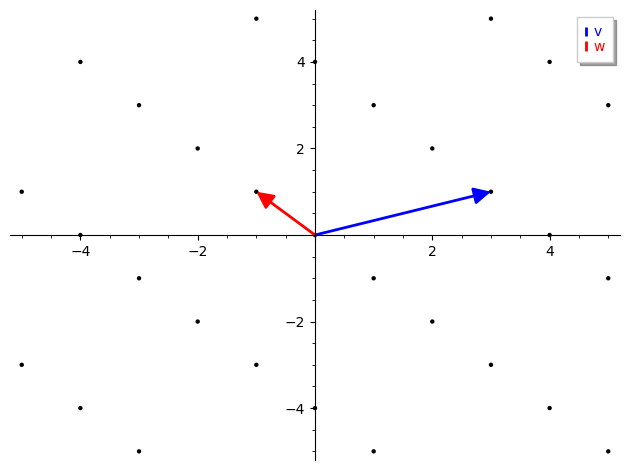
\includegraphics[width=\textwidth]{./img/lattice_b0.png}
        \caption{Lattice $L$ spanned by $v, w$}
        \label{fig:lattice0}
    \end{minipage}
    \hspace{\fill}
    \hspace{\fill}
    \hspace{\fill}
    \hspace{\fill}
    \hspace{\fill}
    \begin{minipage}[b]{0.50\textwidth}
        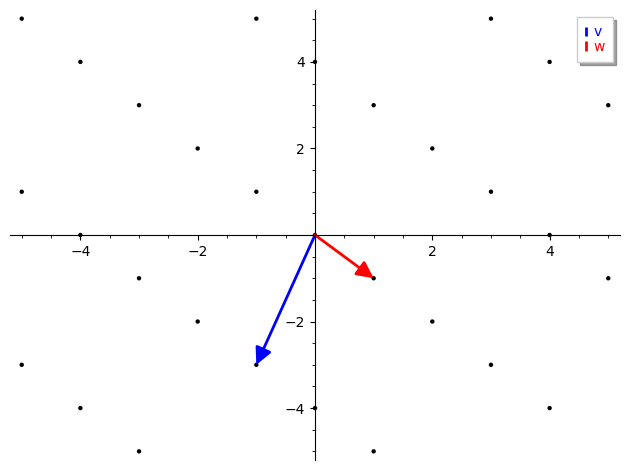
\includegraphics[width=\textwidth]{./img/lattice_b1.png}
        \caption{Lattice $L$ spanned by $v', w'$}
        \label{fig:lattice1}
    \end{minipage}
\end{figure}

\section{Problems}

\subsection{SVP}

\textbf{The Shortest Vector Problem} (\texttt{SVP}): Find a nonzero vector $v \in L$ that minimez the Euclidean norm $\lVert v \rVert$.

\begin{algorithm}
    \textbf{Gauss Reduction}
\end{algorithm}

\begin{figure}[b]
    \centering
    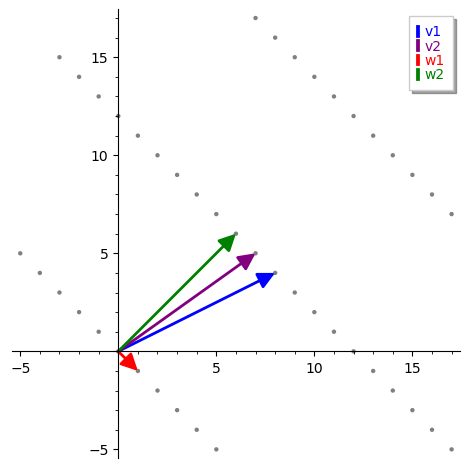
\includegraphics[width=0.5\textwidth]{./img/gauss_svp.png}
    \caption{Gauss reduction}
    \label{fig:gauss_svp}
\end{figure}

Gauss's developed an algorithm to find an optimal basis for a two-dimensional lattice given an arbitrary basis. The output of the algorithm
gives the shortest nonzero vector in $L$ and in this way solves the \texttt{SVP}.

If we take for example $v_1 = (10, 4), v_2 = (7, 5)$ and apply the gauss reduction algorithm we
obtain $w_1 = (3, -1), w_2 = (4, 6)$ \ref{fig:gauss_svp}. $w_1$ is the shortest nonzero vector in the lattice $L$ spanned by $v_1, v_2$.

However the bigger the dimension of the lattice, the harder is the problem and there isn't a polynomial algorithm to find such vector.

\subsection{CVP}

\textbf{The Closest Vector Problem} (\texttt{CVP}): Given a vector $w \in \R^m$ that is not in $L$, find a vector $v \in L$ that is closest to $w$,
in other words find a vector $v \in L$ that minimizes the Euclidean norm $\lVert w - v \rVert$.

Example in \ref{fig:cvp}

\begin{figure}[t]
    \centering
    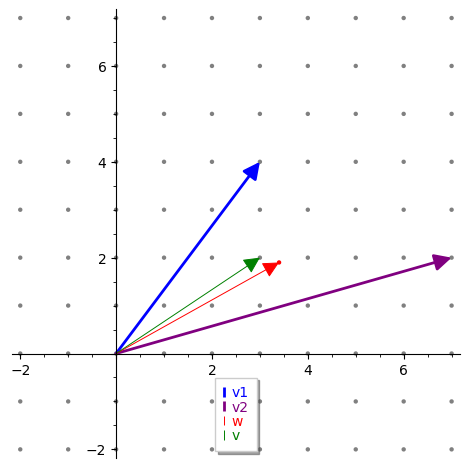
\includegraphics[width=0.5\textwidth]{./img/cvp.png}
    \caption{CVP}
    \label{fig:cvp}
\end{figure}

TODO: CVP and SVP are related.

% matrix([[0, 0, 1], [1, 1, 2], [1, 2, 1]])
\chapter{LLL}

\section{Introduction}

The \textbf{Lenstra-Lenstra-Lovász} \textit{LLL} or \textit{$L^3$} is a polynomial time algorithm to find a "shorter" basis.

\begin{theorem}
    \textbf{LLL}
\end{theorem}

\textit{Let $L \in \Z^n$ be a lattice spanned by $B = \{v_1,\ldots,v_n\}$. The LLL algorithm outputs a reduced lattice
basis $\{w_1, \ldots, w_n\}$ with}

\begin{center}
    $\lVert w_i \rVert \le 2^{\frac{n(n-1)}{4(n-i+1)}} det(L)^{\frac{1}{n-i+1}}$ for $i=1,\ldots,n$
\end{center}

\textit{in time polynomial in n and in the bit-size of the entries of the basis matrix $B$}.\\

Basically the first vector of the new basis will be as short as possible, and the other will have increasing lengths. The new vectors
will be as orthogonal as possible to one another, i.e., the dot product $w_i \dd w_j$ will be close to zero.

\subsection*{Example}

For example we can take the following basis (the rows are the vector) that span
a lattice $L$.

\[
L = 
\begin{pmatrix}
    4 & 9 & 10\\
    2 & 1 & 30\\ 
    3 & 7 & 9
\end{pmatrix}
\] 

Applying the LLL algorithm we obtain

\[
LLL(L) = 
\begin{pmatrix}
    -1 & -2 & -1\\
     3 & -2 &  1\\
    -1 & -1 &  5
\end{pmatrix}
\] 

Where the first row is the shortest vector in the lattice $L$, and so solves the \textbf{SVP} problem.
For higher dimensions however the LLL algorithm outputs only an approximation for the \textbf{SVP} problem.

\section{Algorithm}

TODO: Write algorithm and explain some steps

\section{Applications}

There are many applications of LLL

\begin{enumerate}
    \item Factoring polynomials over the integers. For example, given $x^2 - 1$ factor it into $x + 1$ and $x - 1$.
    \item Integer Programming. This is a well-known \textbf{NP}-complete problem. Using LLL, one can obtain a polynomial time solution
          to integer programming with a fixed number of variables.
    \item Approximation to the \textbf{CVP} or \textbf{SVP}, as well as other lattice problems.
    \item Application in cryptanalysis.
\end{enumerate}

\chapter{Applications}

\section{Attack Knapsack}

\section{Attack RSA}

\chapter*{End of Paper}

$gg^2$

\bibliographystyle{plain}
\bibliography{paper}

\end{document}

